\documentclass[12pt]{report}
\usepackage{textgreek}
\usepackage{fullpage}
\usepackage[final]{pdfpages}

\begin{document}
\title{Intro to Modern Optics uBook}
\author{James Clements}
\date{Fall 2012}
\maketitle
\tableofcontents
\part{Physics of Light}
\chapter{Wave Motion}
Light acts in some ways as a wave and in other ways like a particle (does that make it a wavicle?). Understanding the basics of waves is useful for studying light. We'll examine these first as one dimensional waves to develop some first principles and then expand these fundamentals to apply to two dimensional and three dimensional waves.
\section{One-Dimensional Waves}
This is the easiest way to consider a wave. Consider perturbing a string or a spring by suddenly jerking one end upward and then back to it's original position. This will cause a perturbation to travel through the object. The actual material does not permanently deform as it returns to its original state and thus the disturbance advances and not the medium. The disturbance of a wave is a function of position and time and is denoted by the symbol \textpsi : 
\[\psi (x,t) = f(x,t)\]

The profile of the wave is determined by setting time equal to zero as in: 
\[\psi(x,t)|_{t=0} = f(x,0) = f(x) \]

When considering time, a wave travels at a specific velocity \emph{v}. The distance a wave travels is simply \emph{vt}. An alternate frame of reference, \emph{S'} can be used which travels along with the pulse in time. In this frame, the pulse always looks identical to the profile when \emph{t=0}. Here, the coordinate is \emph{x'} rather than \emph{x} such that $ \psi = f(x') $. The relationship between \emph{x} and \emph{x'} is: $ x' = x - vt $. To describe the wave as someone would observe from the original reference frame, \emph{S}, we can now write that:
\[\psi(x,t) =f(x-vt)\]
This is the general form of the one-dimensional wavefunction. 
\subsection{The Differential Wave Equation}
The differential wave equation is a linear, homogeneous, second order, partial differential equation that is usually taken as the defining expression for physical waves in a lossless medium. The one-dimensional form of the wave equation is derived from the initial relation ship of $\psi(x,t) = f(x')$. Derivatives are taken twice (see Hecht, 4th edition pages 13-14 for details) to bring to the final result of:
\begin{equation}
\frac{\partial ^2\psi}{\partial x^2} = \frac{1}{v^2}\frac{\partial ^2\psi}{\partial t^2}
\end{equation}
This is the wave equation for undamped systems that do not contain sources in the region under consideration. Damping effects would be considered using a $\frac{\partial \psi}{\partial t} $ term.

\section{Harmonic Waves}
Harmonic waves have a sinusoidal profile. Any wave shape can be synthesized by a superposition of harmonic waves, so they're pretty useful. The simplest profile of a harmonic wave can be expressed as: \[\psi(x,t)|_{t=0}=\psi(x) = A\sin kx = f(x)\] where \emph{A} is the amplitude of the wave and \emph{k} is a positive constant known as teh propagation number. Transforming this into a progressive wave yields: 
\begin{equation}
\psi(x,t) = A\sin k(x-vt) = f(x-vt)
\end{equation} 
The symbol $\lambda$ represents the wavelength (also known as spatial period) of the wave and is related to $k$ by the following equation: 
\begin{equation}
k = 2\pi /\lambda
\end{equation}

The amount of time it takes for one complete wave to pass a stationary observer is defined as the temporal period, \texttau . Propagation number, wave velocity, and temporal period are related by the following relationship: \[kv\tau=2\pi\] it also follows that \[\tau=\lambda/v\]

The temporal frequency, \textnu , is the number of waves per unit time (often measured in Hertz) and is related to the above terms under the following equations:
\begin{equation}
\nu \equiv 1/\tau
\end{equation}
\begin{equation}
v = \nu\lambda
\end{equation}

Other related useful terms are the angular temporal frequency, \textomega , and the wave number (spatial frequency), $\kappa$, which are defined respectively as:
\begin{equation}
\omega \equiv 2\pi/\tau = 2\pi\nu
\end{equation}
\begin{equation}
\kappa \equiv 1/\lambda
\end{equation}

Another important note is that no wave is monochromatic, meaning that it has perfect frequency. All waves fall into a band of frequencies. When that band is small, the wave is termed quasimonochromatic. 

\section{Phase and Phase Velocity}
Wave equations are often written in the form: 
\begin{equation}
\psi(x,t) = A \sin (kx-\omega t +\epsilon)
\end{equation}
Wherein the portion inside the sine term consists of the position of the wave, $kx$, the time state of the wave, $\omega t$, and a constant, $\epsilon$ that defines the initial phase of the wave. Without the initial phase, the function would always be zero at the origin of space and time.

Note once again that $\omega$ is the rate of change of phase with time:
\[|(\frac{\partial\psi}{\partial t})_x|=\omega\]
the rate of change of phase with distance keeping t constant is $k$:
\[|(\frac{\partial\psi}{\partial x})_t|=k\]
and the phase velocity, $v$, is the speed at which the wave propagates in space:
\[(\frac{\partial x}{\partial t})_\psi = \pm \frac{\omega}{k} = \pm v  \]

\section{The Superposition Principal (basics)}
Since the differential wave equation is a linear partial differential equation, it holds that the sum of two individual solutions to the wave equation is also a solution to the wave equation. When two separate waves overlap in space, the resulting disturbance at each point in the region of overlap is the algebraic sum of the individual constituent waves at that location. 

Waves are said to be in-phase when their phase angles are identical and can be out of phase to a limit of having a phase angle difference of \textpi. Out of phase waves give rise to interference. 

\section{The Complex Representation}
Euler's formula, $e^{i\theta} = \cos\theta+i\sin\theta$, is often a mathematically optimal way to express harmonic waves since operations such as taking a derivative and multiplying functions is much easier. It is often most convenient to express the harmonic wave as:
\begin{equation}
\psi(x,t) = Ae^{i(\omega t -kx+\epsilon)}
\end{equation}
An important note is that while the imaginary portion of the function is kept out of convenience through calculations, the real part of the equation is the actual expression of the wave. This is only done after obtaining the final result of all calculations.
\section{Phasors and the Addition of Waves}
Phasors are a useful abstraction for understanding waves. Phasor notation contains the amplitude and current phase angle of the wave. Phase angle is the angle by which the wave is offset from its reference state. Phasors are expressed as $$A\angle \phi $$ where $A$ is the maximum amplitude of the wave and $\phi$ is its phase angle. 

When combining wavefunctions, phasors can be used similarly to vectors. The wavefunctions being summed are added head to tail in order to determine the resultant vector. 

\section{Plane Waves}
A plane wave is the simplest example of a three-dimensional wave, but it is extremely useful as all other three-dimensional waves can be described as a combination of plane waves.

Plane waves travel along a propagation vector $\vec{k}$ whose magnitude is the propagation number, k, which has already been described in terms of harmonic waves. The equation of a plane, r, which is perpendicular to $\vec{k}$ is:
\[\vec{k}\cdot\vec{r} = a\] where $a$ is a constant. 

The general equation of a harmonic plane wave in Cartesian coordinates is:
\[\psi(x,y,z,t) = Ae^{i(k_xx+k_yy+k_zz \mp \omega t)}\]

\section{The Three-Dimensional Wave Equation}
The three-dimensional wave equation is extremely similar to the 1-dimensional version. The only difference is that three spatial variables are taken into account. The 3-D wave equation takes on the form:
\begin{equation}
\nabla^2 \psi = \frac{1}{v^2}\frac{\partial\psi}{\partial t^2}
\end{equation}

where $\nabla$ is the Laplacian operator: $\nabla \equiv \frac{\partial ^2}{\partial x^2}+\frac{\partial ^2}{\partial y^2}+\frac{\partial ^2}{\partial z^2}$

\section{Spherical Waves}
Spherical waves represent a point source radiating outward or a spherical shell radiating inward. The harmonic spherical wave equation is given as:
\begin{equation}
\psi (r,t) = \left( \frac{\mathcal{A}}{r} \right)\cos k(r \mp vt )
\end{equation}

\section{Cylindrical Waves}
Cylindrical waves do not have a clean solution to their differential wave equation. Bessel's equation can be used to approximate cylindrical waves of large radii:
\[\psi(r,t) \approx \frac{\mathcal{A}}{\sqrt{r} \cos k(r \mp vt)}\]

This equation best approximates what happens to a plane wave that encounters a long, narrow slit. 

\section{Glossary}
\begin{description}
\item[amplitude:] The maximum disturbance of a wave.
\item[angular temporal frequency:] The number of phase angle changes per unit time, denoted as \textomega .
\item[harmonic waves:] A wave that can be represented using sine or cosine curves. 
\item[in-phase:] Multiple waves having a phase-angle difference of zero are in phase. The disturbance of the waves sums maximally causing a much greater intensity resultant wave.
\item[initial phase (\textepsilon ):] The angle which is the constant contribution to the phase arising at the wave generator. This is independent of how far in space or how long in time the wave has traveled. 
\item[longitudinal wave:] A wave in which the  medium is displaced in the direction of the motion of the wave.
\item[monochromatic:] A wave which travels at constant frequency.
\item[out-of-phase:] Multiple waves having a phase-angle difference of 180$^{\circ}$ are said to be out of phase. The waves interfere with each other such that the resultant wave disturbance is minimized. 
\item[phase velocity:] The speed at which a wave profile moves. Denoted as $v = \frac{\omega}{k}$.
\item[phasor:] An abstraction useful in expressing a harmonic wave in terms of its amplitude, \emph{A} and phase, $\phi$ as $A \angle \phi$. 
\item[plane wave:] A planar wave that is perpendicular from a direction vector, $\mathbf{\vec{k}}$.
\item[propagation number:] A positive constant denoted as \emph{k} used in studying harmonic waves which ensures correct units inside the sine function and can change the period of the sine wave. When \textlambda  is defined as the wavelength, $k=2\pi /\lambda$.
\item[spacial frequency:] The number of waves per unit length, denoted by $\kappa$. Synonymous with wave number. 
\item[superposition principle:] The principle in which multiple waves traveling along the same path are summed. 
\item[temporal frequency:] The number of waves per unit time, denoted as \textnu. Often takes on units of Hertz (Hz). 
\item[temporal period:] Denoted as \texttau. This is the amount of time it takes for one complete wave to pass a stationary observer.
\item[transverse wave:] A wave in which the medium is displaced in a direction perpendicular to that of the motion of the wave
\item[traveling wave:] A wave whose crest travels across particles.
\item[wavefront:] The surfaces of a three-dimensional wave that join all points of equal phase. 
\item[wave number:] The number of waves per unit length, denoted by $\kappa$. Synonymous with spacial frequency. 
\end{description}
\section{Important Equations}
\[\frac{\partial ^2\psi}{\partial x^2} = \frac{1}{v^2}\frac{\partial ^2\psi}{\partial t^2}\]
\[\psi(x,t) = A\sin k(x-vt) = f(x-vt)\]
\[k = 2\pi /\lambda\]
\[\nu \equiv 1/\tau\]
\[v = \nu\lambda\]
\[\omega \equiv 2\pi/\tau = 2\pi\nu\]
\[\kappa \equiv 1/\lambda\]
\[\psi(x,t) = A \sin (kx-\omega t +\epsilon)\]
\[\psi(x,t) = Ae^{i(\omega t -kx+\epsilon)}\]
\[\nabla^2 \psi = \frac{1}{v^2}\frac{\partial\psi}{\partial t^2}\]
\[\psi (r,t) = \left( \frac{\mathcal{A}}{r} \right)\cos k(r \mp vt )\]

\section{Homework Problems}

Due October 4, 2012.

Problems from Hecht Optics Chapter 2: numbers: 4, 13, 17, 18, 22, 32
Solutions were hand written and are shown on the following pages. 
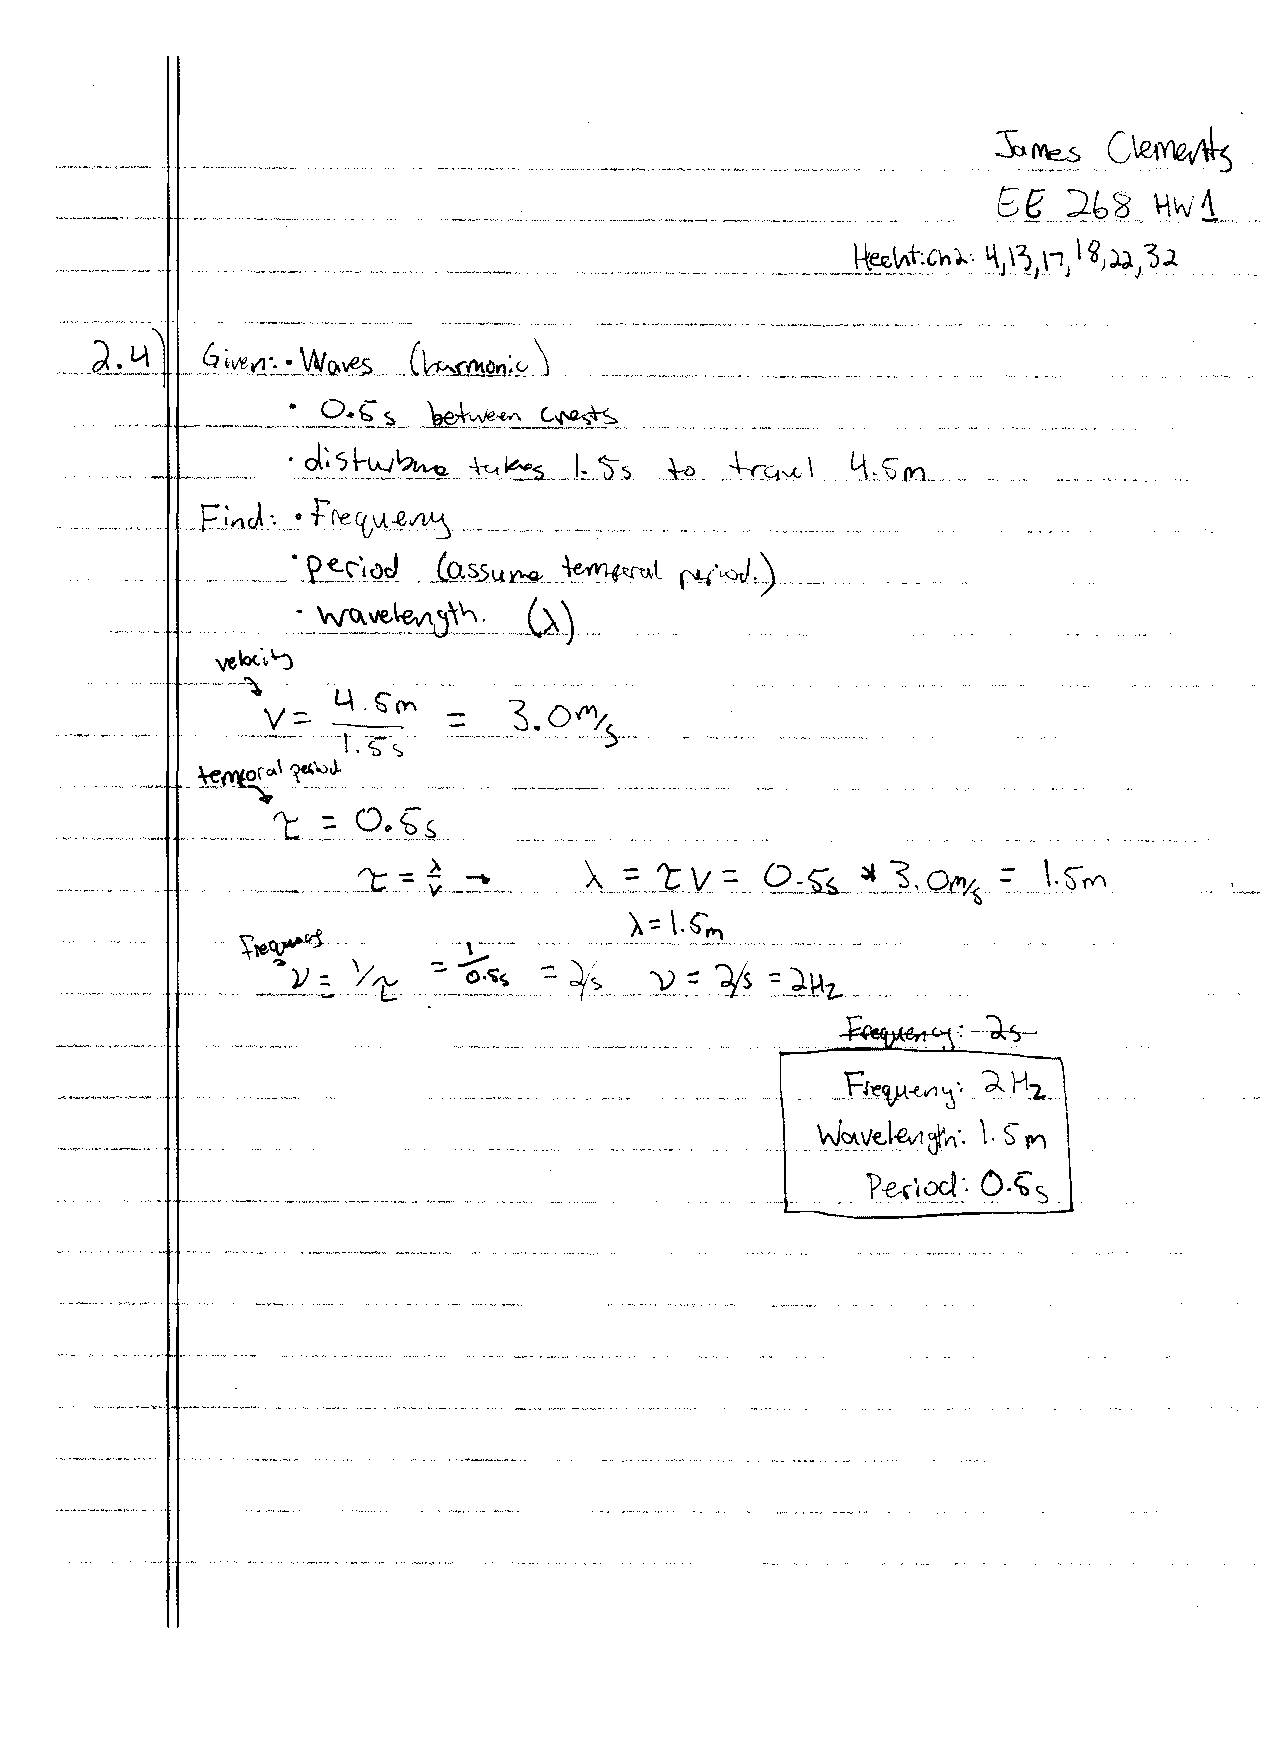
\includepdf[ pages=- ]{EE268HW1}


\chapter{Superposition of Waves}
\chapter{Electromagnetic Theory, Photons, and Light}
\chapter{Polarization}
\chapter{Interference}
\chapter{Modern Optics - Lasers and Such}



\part{Light and Matter}

\chapter{The Propagation of light}
\chapter{Diffraction}
\chapter{Basics of Coherence Theory}

\part{Analysis Techniques}
\chapter{Geometrical Optics}
\chapter{More on Geometrical Optics}
\chapter{Fourier Optics}


\end{document}
